% !TeX encoding = UTF-8
\chapter{Analysis and Implementation}
\label{chap2}

In this chapter we analyze the algorithm used to process EBSD data and explain how to implement it effectively for GPUs. We use the CUDA platform, which is currently the most popular technology for general purpose computing on graphics cards.

The input for the algorithm consists of one reference and many deformed backscatter patterns which are captured in greyscale images. There may be up to tens of thousands of them. In general, the format of the pictures is not important, as long as it is possible to load them from disk quickly. For example, our testing data consists of 15000 images saved in TIFF format without any compression. Each picture has resolution of approximately $900 \times 900$ pixels and each pixel is represented by a 16 bit unsigned integer --- the higher the integer, the higher is the luminosity of the pixel.

The result of the algorithm is a list of two--dimensional vectors that we write to the standard output.

There are further parameters to the algorithm explained in the \cref{chap1}. \Cref {params} summarizes them along with the range of values that we consider. The size of input pattern range is based on the resolution of commonly accessible EBSD cameras \cite{digiview-ebsd-camera} \cite{hikari-ebsd-camera}. Our testing data resolution is also within this range. The range of rest of the parameters is based on consultation with physicists from Department of Physics of Material in Charles University in Prague.

\begin{table}[]
	\centering
	\begin{tabular}{@{}lll@{}}
		\toprule
		Parameter                  & Label            &    Value range  \\ \midrule
		Size of input pattern      & $W_p \times H_p$ & $640 \times 480$ -- $1400 \times 1000$  \\
		Number of subregions       & $S$              &               10 -- 100 \\
		Size of a subregion        & $W_r \times H_r$ & $50 \times 50$ -- $250 \times 250$ \\
		Diameter of a neighborhood & $F$              &                3,5,7,9 \\ \bottomrule
	\end{tabular}
	\caption{Summary of algorithm parameters with example values that show their order of magnitude.}
	\label{params}
\end{table}

In the following sections, we first explain the computation of cross--cor\-re\-la\-ti\-on, sum and arg max on the GPU. Then, algorithm, we explain how they are used together to implement the algorithm outlined in chapter 1. We can divide it into 2 major parts: first, preprocessing of the images prior to cross--correlation that includes loading the image from disk and subtracting sums of the subregions, which is addressed in \cref{preprocessing}. Second part, described in \cref{cross-processing}, consists of processing of its result, which includes search of the maximum position and finding the maximum within each neighborhood.

The most important feature of the algorithm upon which we build our GPU implementation is the fact that all the subregions are completely independent from each other. So every kernel described in the following sections processes all the subregions of a pattern in parallel (we also implemented batch parameter described in \cref{batch-param}, which allows processing more images at once). This way, we can make sure we utilize the whole GPU. 

\section{Cross--correlation}
We start by analyzing the core of the algorithm --- cross--correlation, which is also the most computationally demanding part. The input for cross--correlation are two images, in our case it is a deformed and a reference subregion. More precisely, there are several pairs of subregions, but since they are completely independent, we explain the algorithm for one pair only. With respect to the definition in \cref{cross-corr-def}, we cross--correlate the reference with deformed subregion, i.e. $reference \star deformed$, not the other way around. Also, both subregions are of the same size, which simplifies some aspects of the algorithm.

\subsection{Related work}

Since cross--correlation is quite a common operation in image processing, various researchers implemented it on GPUs. For example, Liu, Zou and Luo implemented the cross--correlation for CUDA 3.1 using the cuFFT library in 2011 \cite{liu2011gpu}. Lewis explained how to optimize computation of normalized cross--correlation denominator \cite{lewisfast} and Gangodkar et al. implemented it for GPU \cite{gandokar2012fastNCCGPU}. It is also used as part of various image processing algorithms, for example Idzenga, Gaburov, Vermin, Menssen and De Korte used a GPU implementation of normalized cross--correlation for ultrasound images analysis \cite{Idzenga2014Ultrasonics}.

There are also libraries that can leverage GPUs to compute cross--cor\-re\-la\-tion. Matlab has a function called \texttt{xcorr2} that can be GPU--accelerated \cite{MATLAB:2018}. The NPP library with C interface by NVIDIA \cite{NPP} also contains a function to compute two--dimensional cross--correlation. However, none of the libraries we managed to find offers a possibility to process batches of images. Since we process a large amount of rather small images, there would be unnecessary overhead of many library function calls that do only a small amount of work.

\subsection{Definition--based algorithm}
We first describe a naive algorithm designed directly from the definition. Then we explain another one that uses discrete Fourier transform. The reason why we implement two versions is that although the Fourier transform based algorithm has better asymptotic complexity, the subregions may not be big enough to reflect it.

A serial algorithm for cross--correlation is shown in Algorithm \ref{crossAlgo}. It is directly based on the definition. It iterates over all possible shifts between the images (subregions), i.e. $\forall [shiftX, shiftY] \in [-W_s+1, W_s-1] \times (-H_s, H_s)$. For each of the shifts $[shiftX, shiftY]$, we sum over the products of pixels that overlap when we shift the deformed subregion by shiftX pixels horizontally and by shiftY vertically.


\begin{algorithm}
	\caption{Serial algorithm that computes cross--correlation.}
	\label{crossAlgo}
	\KwIn{reference: an array of pixels of a reference subregion \newline
		deformed: an array of pixels of a deformed subregion \newline
		$W_s, H_s$: size of both subregions}
	\KwOut{result: cross--correlation between reference and deformed subregions}
	\vspace{5px}
	
	\For{$\text{shiftX} \in [-W_s+1, W_s-1]$}{
		\For{$\text{shiftY} \in [-H_s+1, H_s-1]$}{
			sum = 0\;
			\For{$x \in [0, W_s-1]$}{
				\For{$y \in [0, H_s-1]$}{
					shiftedX = x + shiftX\;
					shiftedY = y + shiftY\;
					\If{$\text{shiftedX} \in [0,W_s-1]$ \textbf{and} $\text{shiftedY} \in [0,H_s-1]$}{
						sum += reference[x,y] * \newline deformed[shiftedX, shiftedY]\;
					}
				}
			}
			result[shiftX, shiftY] = sum\;
		}
	}
\end{algorithm}

\begin{algorithm}
	\caption{Pseudocode of CUDA kernel that computes cross--correlation.}
	\label{crossKernel}
	
	shiftX = threadId.x\;
	shiftY = threadId.y\;
	intervalX = $[max(-shiftX, 0), min(W_s - shiftX, W_s) - 1]$\;
	intervalY = $[max(-shiftY, 0), min(H_s - shiftY, H_s) - 1]$\;
	
	sum = 0\;
	\For{$x \in [max(-shiftX, 0), min(W_s - shiftX, W_s) - 1]$}{
		\For{$y \in[max(-shiftY, 0), min(H_s - shiftY, H_s) - 1]+$}{
			shiftedX = x + shiftX\;
			shiftedY = y + shiftY\;
			sum += reference[x,y] * deformed[shiftedX, shiftedY]\;
		}
	}
	result[shiftX, shiftY] = sum\;
	
\end{algorithm}

The inner two loops of the algorithm iterate through all pixels of the reference image. However that is not necessary for all shifts, since for most of them only smaller parts of the images overlap (the only shift that requires iteration through all points is $[0,0]$). The if statement then filters out the pixels that do not overlap for specific shift. For performance reasons, we can get rid of the if statement, if we rewrite the two inner loops to always stay within the boundaries of the images.

We will only reason about $shiftX$, since the same argumentation applies to $shiftY$. So we need to find out for which $x \in [0, W_s - 1]$ holds that $(x + shiftX) \in [0, W_s-1]$, if $shiftX \in [-W_s+1, W_s-1]$. The result is the following interval:
\[
x \in [max(-shiftX, 0), min(W_s - shiftX, W_s) - 1].
\]
This gives us an interval through which we iterate $x$ in the inner loops for each \IT{shiftX}. Similar modification applies for the y loop based on \IT{shiftY} as well.

The modified algorithm written as a CUDA kernel is listed in algorithm~\ref{crossKernel}. We implemented the algorithm for CUDA by parallelizing over the outer two loops. That means each thread computes one shift and thus one value of the result. It uses two--dimensional blocks, so we can just use the two indices as \IT{shiftX} and \IT{shiftY}. For computing more subregions at a time, we simply use more threads.

\subsection{The cuFFT library}
We now move on to explain our implementation of the cross--correlation computation using the Fourier transform. We use the cuFFT\footnote{\url{https://docs.nvidia.com/cuda/cufft/index.html}} library for CUDA to compute the discrete Fourier transform and its inverse. It is a highly optimized implementation of the \emph{Fast Fourier algorithm}, which computes the Fourier transform in time $\mathcal{O}(n \log n)$. It also supports batched transformations (i.e. several unrelated transformations can be done by calling a single library function), which is very important for our implementation, since we do many transformations of rather small images at once. In this section, we explain the implementation for one subregion only, since it is trivial to expand it for more subregions.

There are two functions in the cuFFT library that are essential for us \texttt{R2C} and \texttt{C2R}, which compute the discrete Fourier transform and its inverse, respectively. \texttt{R2C} takes an array of real numbers and computes their discrete Fourier transform, outputting an array of complex numbers. A complex number is represented as a pair of floats/doubles. The \texttt{C2R} function takes an array of complex numbers, computes their inverse Fourier transform and outputs an array of real numbers.

Both of the functions use an important property of Fourier transform: A series $x$ of $N \in \mathbb{N}$ numbers is real-valued if and only if the Fourier transform of $x$ denoted as $X$ satisfies the Hermitian symmetry, e.g. $X_k = X_{N-k}^\star$. So it is enough to store just half of the transformed array, since the second half can be trivially computed. cuFFT does just that. Analogous theorem applies to two--dimensional Fourier transform as well, so cuFFT operates on roughly half of the elements, namely on the elements with index from the following set: $\{0,1,\cdots, \floor{W/2} + 1\} \times \{0, 1, \cdots, H\}$, where $H$ is number of rows and $W$ is number of columns of the input matrix.

It also makes it possible to store the Fourier transform in roughly the same array as the input and thus perform in--place transforms. The output consists of complex numbers, which are represented by two real numbers, i.e., one element takes twice as much bytes. But at the same time, we only need $W/2 + 1$ columns (we can remove the floor operator, because $W$ is always even in our context as we double the size of a subregion with zero padding). The result is that we save the input in a real matrix with size $(W+2) \times H$, with the two extra columns unused. That is the same amount of space that we need for the transformed complex matrix with size $W/2 + 1 \times H$.

\subsection{Using cuFFT to compute cross--correlation}
\label{FFT-cross-corr-impl}

We need to cross--correlate a reference and a deformed image. Recall that it can be computed in several steps explained in \cref{two-dim-ft}:

\begin{enumerate}
	\item Zero--pad the images.
	\item Compute the Fourier transforms of the images, which gives us two matrices $X = \mathcal{F}(x)$ and $Y =\mathcal{F}(y)$.
	\item Multiply $X^\star$ with $Y$ element by element.
	\item Do the inverse discrete Fourier transform on the product.
	\item Swap quadrants of the result.
\end{enumerate}

We use cuFFT functions described in previous section to perform steps 2 and 4. The step 3 requires a custom kernel. The first and the last step depend on the remaining ones and we show how to optimize them out below.

We have only one reference image that is cross--correlated with all the deformed ones. So we can prepare the reference subregions by executing the first two steps only once and just read from the prepared buffer in step 3 during processing of all the deformed images. 

The cuFFT functions have both an in--place version, which is used when the input and output buffers are the same, and out--of--place version, which is used for different input and output buffers. Using the out--of--place has the disadvantage if allocating multiple buffers --- one for input zero--padded data, one for transformed matrix and one for the output. However there are two advantages: first, the out--of--place versions of the cuFFT functions proved to be slightly faster. Second, it is possible to preserve the zero padding created by the first step when using the out--of--place version. The zero--padding can be written only once for the first image and then every time we load a new image (prior to the cross--correlation computation), we overwrite the same portion of the buffer with new deformed subregion. All the subregions are of the same size, so the same portion of the buffer is used every time. Since memory consumption is not an issue with our implementation, we can afford to allocate more buffers so we consider the out--of--place version better.

For the step 3, we implemented a kernel that does the element--wise multiplication between the complex conjugate of the Fourier--transformed reference subregion and the Fourier transform of deformed subregion. The result of the multiplication can be outputted to the buffer with Fourier transform of the deformed subregions, since we do not need it any more. Implementation of the kernel is quite straightforward, each thread loads two complex numbers, multiplies them and writes them back. It can benefit from the batch parameter (see \cref{batch-param}) --- since we process several deformed subregions in one kernel call, we can load the complex number from reference subregion only once and use it multiple times.



Then we compute the inverse Fourier transformation using the \texttt{C2R} function from the cuFFT library. The result is the cross--correlation, but with extra row and column of zeros and swapped quadrants as described in \cref{two-dim-ft}.

\Cref{fft-impl} shows all the steps with illustration of used buffers. The input image has size $W_s \times H_s$, but it has to be inside a buffer with size $2W_s \times 2H_s$ to accommodate the zero padding. The transformed image has the size $(W_s+1) \times 2H_s$ complex numbers, which is the same as  $(2W_s+2) \times 2H_s$ of real numbers. The same--sized buffer is needed after the multiplication. Then we perform the inverse Fourier transform to get the cross--correlation with swapped quadrants (as described in \cref{two-dim-ft}).

\begin{figure}
	\centering
	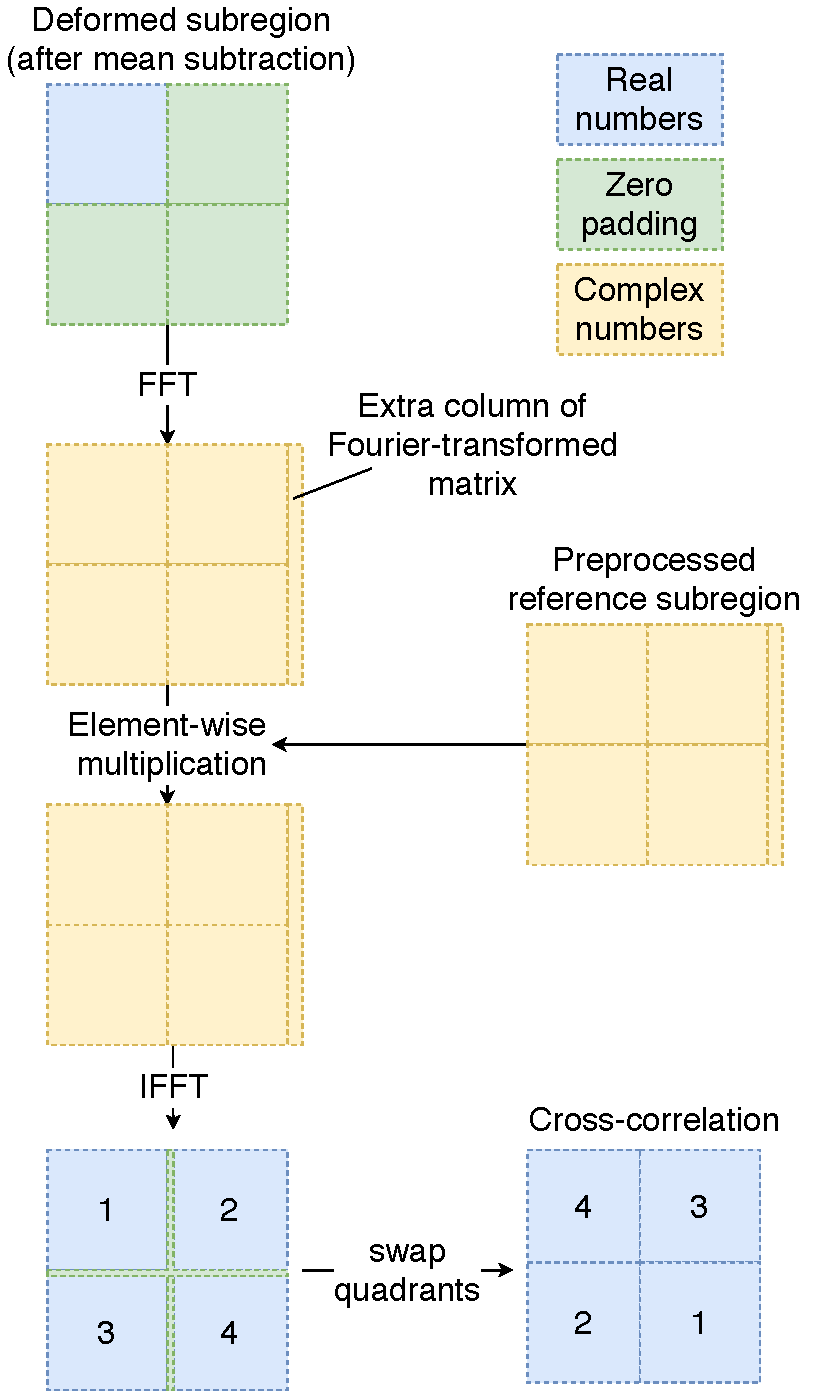
\includegraphics[width=0.7\textwidth]{img/fft-impl}
	\caption{The process of computing cross--correlation using the discrete Fourier transform.}
	\label{fft-impl}
\end{figure}

The last step to get the cross--correlation is to swap the quadrants of the result. The most straightforward solution is to start a kernel which does just that and thus finalizes the cross--correlation. Such kernel moves a considerable amount of data around and thus is relatively expensive. Instead, we can modify the rest of the implementation, so it accesses the data in corresponding way. In the next steps, we need to find the position of the maximal value in the cross--correlation and then process the neighborhood of the maximum. It can be easily modified to work with incomplete cross--correlation with swapped quadrants. The search of maximum stays the same and outputs the position of maximum, which then has to be interpreted correctly when fetching the neighborhoods to process them. This trick removes the overhead of running the extra kernel at the cost of more complicated, but only slightly more demanding data address calculation. Moreover, it works with much less amount of data, as the neighborhoods are only a small part of the cross--correlation.

\vspace{5px}

To sum up, we have described two ways to compute cross--correlation. The first one is based on the definition, the second one uses the Fourier transform which makes it possible to achieve better asymptotic time complexity. However for smaller input sizes, the definition--based approach is faster --- we measure that in chapter 3.


\section{Sum computation}
\label{sums}

Computation of sum is a textbook example of parallel reduction. In \cite{parallelReduction}, Justin Luitjens explains how to implement it on modern GPUs. Since it is very expensive to communicate between arbitrary threads during computation, the reduction is separated into three steps: first, each thread loads several values and computes their sum, then we reduce the data within each block individually and finally we synchronize single value for each block. The major difference for our case is that we compute a sum for each of several subregions, instead of reducing over the whole input data. The problem is that we cannot load values of two different subregions into one block. We solve this by assigning whole blocks to the subregions rather than just assigning threads to pixels.

Let $K$ be number of values that each thread loads, $B$ denote one block size and $P$ total number of pixels in one subregion, respectively. Then we use a group of $S_1~=~\ceil{\frac{P}{KB}}$ blocks for reduction of each subregion. If $P$ is not divisible by $KB$, then the last block in each group is not fully utilized, and processes only $K - 1$ values because there are no more pixels in the subregion.



Once each thread loads its data, it is possible to reduce them fast within each block. We use warp--level shuffle instructions, which allows the threads in one warp to exchange data in registers. \Cref{warp_reduce} shows how it is possible to get sum of values in 8 threads. It can be expanded to size of warp, i.e. 32 threads. To reduce the whole block, we use the warp reduction in two steps:
\begin{enumerate}
	\item We perform the reduction within each warp and save the values into shared memory.
	\item One warp loads the values from the shared memory and reduces them using warp--level reduction again
\end{enumerate}
Maximum number of threads in one block is 1024 in CUDA and warp size is 32 so we get at most $1024/32 = 32$ values in the first step. That means one warp is enough to reduce them into one resulting value in the second step.

\begin{figure}
	\centering
	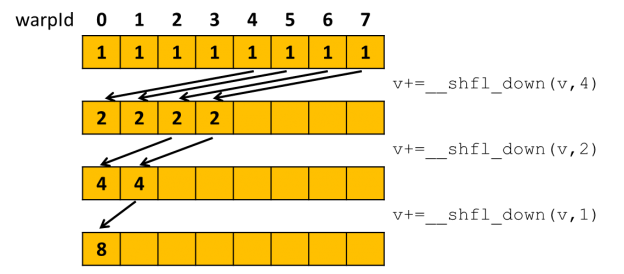
\includegraphics[width=0.7\textwidth]{img/warp_reduce}
	\caption{An example of warp--level reduction for 8 threads \cite{parallelReduction}. \emph{warpId} is a number of thread within its warp.}
	\label{warp_reduce}
\end{figure}

After the reduction within each block, we need to update the resulting values in global memory. If $S_1$ is equal to $1$, thus every subregion is processed by exactly one block, then there is no synchronization needed between the blocks. Otherwise, we can use \emph{atomic add}. The solution is feasible for us, since it is safe to assume that not many blocks access the same value. The worst case size of one subregion is $250 \times 250$ which is the total of 62500 pixels. \XX{ For $K = 1$ and $B = 1024$ (there is no reason not to use the maximal possible value --- no register or shared memory pressure), then 63 blocks compute the sum of one subregion.}. 

We measure the impact of the parameters in section ??. Higher $K$ helps utilize the threads better, because they manage to do more work before the reduction phase. For $K = 1$, half of the threads do (almost) nothing useful in the whole reduction: each of them only loads one value in the very beginning and immediately passes it to another thread (using shuffle instruction) which does the actual sum. On the other side, setting $N$ and $B$ such that only one block processes one subregion can lead to not being able to utilize whole gpu, if there are not enough subregions.


\section{Arg max computation}
\label{arg-max}
The cross--correlated data are further processed to find the position of maximum for each subregion by using parallel reduction. The computation is very similar to the sums reduction explained in \cref{sums} we use warp--level shuffle instructions and shared memory to reduce the values loaded to each block. The difference compared to sum reduction is that we need to find the maximum and its position at the same time. So throughout the algorithm, we operate on the pair of value and its position. Every time we compare two values and choose the higher one, we propagate its position as well.

Otherwise the reduction within one block is analogous to the sum reduction. In each step we shuffle down the current value and its position (that means two shuffles per one step). Then we compare the received and current value and save the greater one with its position for the next step. We need five these steps to reduce one warp, then each warp saves its result to the shared memory. Finally, one warp reduces the items in the shared memory to get the result of one block reduction.

In the sums reduction kernel, we used built-in atomic add to update the global memory with the result of block reduction. No such function exists for arg max, since we need to atomically compare two values and then update the position as well. There are several ways how do the update without the atomic operation.
\XX{
\begin{description}
	\item[Launch second kernel] The first kernel does no synchronization between the blocks and each block just writes its reduced result to its reserved place in global memory. Then, we start second kernel which reduces the results of the first one. In the second kernel, all the values from one subregion are reduced by one block, so there is no synchronization needed anymore. 
	\item[One block reduces one whole subregion] We increase the number of values that each thread loads before the reduction, so only one block is needed to find the maximum of each subregion. Therefore, no synchronization across blocks is needed. Depending on the number of subregions, there is a possibility that this approach does not spawn enough blocks to fully utilize the GPU.
	\item[Atomic compare and swap (float data only)] We can use the atomic compare and swap (CAS) instruction to update the global memory atomically. There are not many blocks that would compete over the same piece of memory, so it is a viable solution. However, it can only be done when we compute the cross--correlation in single precision floating point type, since modern GPUs only support atomic CAS for 8 bytes. A double precision number is 8 bytes long itself, and we need to update the pair of value and its position. 
\end{description}
}
\todo{atomicMax + CAS pristup, ktory by mal fungovat vo vsetkych pripadoch}
The different approaches are compared in chapter 3.



\section{Subregions preprocessing}
\label{preprocessing}
Once we have described the most important parts of the algorithm, we explain how they are used together. In the following section, we outline the preprocessing that is needed before we can cross--correlate the subregions. It incorporates several steps:
\begin{enumerate}
	\item Load an image of pattern from disk
	\item Transfer the image from host memory to GPU memory
	\item Extract the subregions of interest from the image
	\item Compute the sums of subregions
	\item Compute a mean for each subregion and subtract it
\end{enumerate}
In the end, all the image subregions specified by the user are organized one after another in the output buffer on the GPU. In case of cross--correlation implemented by FFT, the subregions are organized in a 4 times larger buffer with zero padding, so that it can be used by the forward Fourier transformation (see \cref{FFT-cross-corr-impl}).

It is not immediately clear, in what order we should perform these steps and which ones should be executed on the GPU. Naturally, load of the image from disk must come first and computation of sums must come before they are subtracted. Also, the image has to be loaded from the disk using CPU, while the rest can be implemented on GPU (the transfer step is of course special in this regard).

First, we decide whether we transfer the whole image and then extract subregions on the GPU, or extract using CPU and transfer only the subregions. If there are only few subregions, the latter approach may transfer less data, since some areas of the pattern are never used. On the other hand, if there are many subregions, they are likely to overlap, which means we could transfer more data than needed. That said, the difference of amount of data transferred does not really matter, since empirical testing showed the time needed to copy the data from host memory to GPU is marginal compared to the rest of the algorithm. However what matters is, that we can utilize GPU for subregion extraction when we, so we have chosen that approach.

The most straightforward GPU implementation of the preprocessing is to write three kernels which first extract the subregions from the image, then compute their sums and finally subtract the means them. We can optimize it by merging the first and the final step --- we first compute the sums by reading the subregions directly from the image of pattern. Then, in the second kernel called \emph{prepare kernel}, we load the pixels of subregions from the image again, compute the mean of respective subregion and subtract it from each pixel. Finally, we write it to proper place in the output buffer. This approach saves us the overhead of starting one kernel

The output of the kernel are the normalized subregions stored in one buffer that is prepared to be cross--correlated. In case of using cross--cor\-re\-la\-ti\-on implementation based on the definition, the subregions are stored continuously side by side. In case of the FFT implementation, the subregions are stored in a continuous buffer of matrices with size $2W_s \times 2H_s$ (one subregion has the size $W_s \times H_s$), each subregion taking the left upper part of the matrix. The rest of the matrices are used for zero padding.

If some subregions are overlapping, we copy some of the data twice, but then we subtract different means from them in general, so the result does not have any duplicities.

The load of the image is implemented using the C library libTIFF \cite{libtiff}. Although TIFF format offers more options for encoding pictures and even compression, the testing images we received (that were produced by an EBSD camera) use simple layout without any compression which is preferable from the performance point of view. The specific testing images are divided into strips of 4 rows, which is roughly 7 kilobytes. Within the strip, the pixels are organized in row-major order, each pixel is represented by an unsigned 16 bit integer. Thus, we are able to load the strips one by one to the host memory without any major performance penalty.

The implementation of kernel that computes sums is described in \cref{sums}. The implementation of the prepare kernel is fairly straightforward, we assign one thread to each pixel in each subregion. The threads compute the position of their pixel in the pattern using the buffer with the positions of the subregions, then compute mean using the sums buffer, subtract it and finally write the value to the output buffer.


\section{Cross--correlation processing}
\label{cross-processing}
After the cross--correlation is finished, we analyze the result --- we find where is the maximum of each subregion using parallel reduction, which is explained in \cref{arg-max}. The result is an array of coordinates of the maximum values (we are not interested in the values themselves). The next kernel then extracts a square shaped neighborhood of each maximum into one continuous buffer, so it can be transferred to the CPU memory together with the positions of the maxima.

\subsection{Extract neighbors kernel}

Once we compute the position of cross--correlation maximum for each subregion, we need to transfer the maxima and their neighborhoods from GPU to main memory so that the CPU can finalize and output the offsets. The maxima are already ready to transfer as a result of the arg max kernel, but we need to start another kernel to copy the neighborhoods from the cross--correlation into its own buffer, so we do not have to transfer the whole cross--correlation.

Recall that $F$ denotes the size of the square neighborhood. Given a maximum $[x_m, y_m]$, its neighborhood are the points $\{x_m - \frac{F-1}{2}, \cdots, x_m, \cdots, x_m + \frac{F-1}{2}\} \times \{y_m - \frac{F-1}{2}, \cdots, y_m, \cdots, y_m + \frac{F-1}{2}\}$ of cross--correlation. $F$ is always an odd number, so that the maximum is in the middle of the neighborhood. So the output buffer has size $F^2 \cdot S$, because each neighborhood has $F \cdot F$ points and there are $S$ subregions.

In the kernel, we assign one thread to each point of the neighborhood. Each thread computes the address of its point and copies it from the cross--correlation buffer to the neighborhoods buffer.

This kernel works with very small amount of data compared to other kernels, since $F$ is expected to be less than 10. Therefore the running time of this kernel is marginal and does not offer much space for improving overall running time.


\subsection{Offsets finalization}
\label{offsets-finalization}
When we have the positions of maxima and their neighborhoods lined up in two buffers, we use the least squares method to fit a quadratic function to the neighborhoods and find the maximum of the resulting continuous function. As shown in \cref{estimation} and \cref{max-fitted}, it all comes down to one matrix--vector multiplication and then solving a simple two variable linear system.

The amount of data processed in this stage of computation is much smaller compared to the rest of the algorithm. In the worst case, i.e. the biggest size of neighborhood $F \times F = 9 \times 9$ that we consider and the smallest size of subregion $W_s \times H_s = 5 \times 50$, the neighborhoods are 30 times smaller than whole subregions. In addition, the offset finalization is not particularly computationally demanding and we empirically measured that in the worst case it takes less than 1\% of the whole algorithm run time. Moreover, it is possible to perform the stage on the CPU in parallel with GPU computation, thus removing its impact on the total time whatsoever, as explained below in \cref{task-paralelization}. Those are the reasons we decided it is pointless to implement it for GPU. However in case the range of considered parameters change in the future, the addition of GPU implementation would not be a problem.

So when we have the positions of maxima and their neighborhoods, we transfer them to the host memory, since the finalization of the offsets takes place on the CPU. Next step is to fit a quadratic function to each neighborhood. As explained in \cref{subpixel-peak}, we have precomputed the matrix $(A^TA)^{-1}A^T$ for each considered $F \in \{3, 5, 7, 9\}$. Then we multiply the neighborhood as a vector with this precomputed matrix using standard matrix multiplication. That results in 6 coefficients of the quadratic function.

Then we use the formulas from \cref{max-fitted} to compute the maximum of the continuous function given by the 6 coefficients, which gives us offset of the maximum from the middle of each neighborhood. In the final step, we combine the location of neighborhoods transfered from the GPU with the relative offsets and write out the result.


\section{Data flow}

\Cref{overview} summarizes the whole algorithm and shows all the used kernels and buffers (apart from additional buffers that are used to compute the cross--correlation).

\begin{figure}
	\centering
	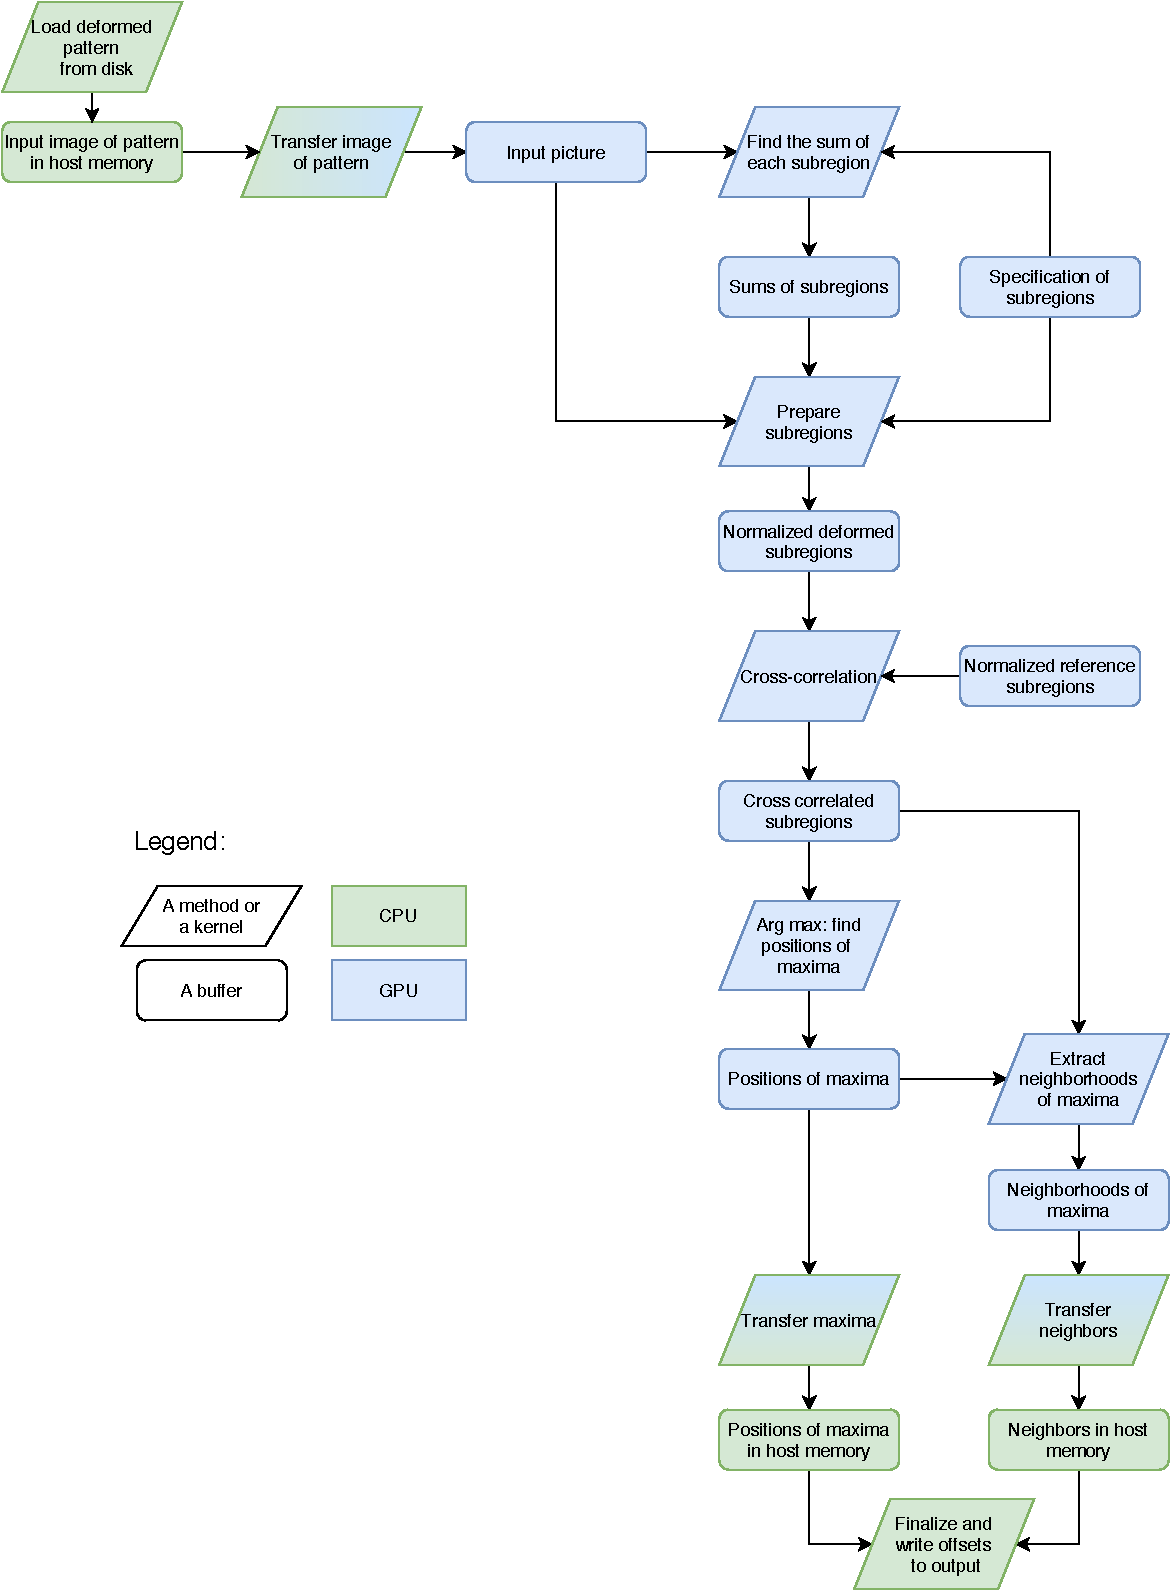
\includegraphics[width=\textwidth]{img/overview}
	\caption{Processing of one deformed pattern.}
	\label{overview}
\end{figure}

\Cref{buftypes} shows all buffers used on GPU with their sizes. The kernels that compute sums and normalize the subregions both work with $W_r \cdot H_r \cdot S$ items (i.e. all subregions). The cross--correlation has nearly four times as big output, which is then processed by the arg max kernel. So the cross--correlation and the arg max kernel work with the largest amount of data, while the buffers that are transferred to the CPU memory are quite small.


\begin{table}[]
	\begin{tabular}{@{}lll@{}}
		\toprule
		Buffer                          & Type         & Number of elements             \\ \midrule
		Input picture                   & uint16       & $W_p \cdot H_p$                \\
		Sums of subregions              & uint32       & $S$                            \\
		Positions of subregions         & uint32 pair  & $S$                            \\
		Normalized deformed subregions  & float/double & $W_r \cdot H_r \cdot S$        \\
		Normalized reference subregions & float/double & $W_r \cdot H_r \cdot S$        \\
		Cross--correlated subregions    & float/double & $(2W_r-1)\cdot(2H_r-1)\cdot S$ \\
		Positions of maxima             & uint32 pair  & $S$                            \\
		Neighborhoods of maxima         & float/double & $F^2 \cdot S $                 \\ \bottomrule
	\end{tabular}
	\caption{Summary of GPU buffers with their data types and size.}
	\label{buftypes}
\end{table}



The \cref{buftypes} also shows the data types stored in the buffers. The input image consists of unsigned 16 bit integers, since that is the format of our testing images. Four byte unsigned integer is then enough to hold the sums of its subregions of expected size.

Once the means are subtracted, the pixels are not integers in general, so we need to use a floating point type. We implemented the algorithm for both single or double floating point types, since the single precision version is substantially faster, but we are not sure whether its precision is sufficient. The result of the algorithm is further processed and the resulting rotation of the pattern is expressed in quite small numbers (in the order of $10^{-4}$), thus small imprecisions introduced by smaller floating point types might matter. That is also why we did not implement the algorithm for half float, but if the 4 byte float proves sufficient, half float may be worth implementing in the future.

\section{Image batch processing}
\label{batch-param}

The algorithm we explained so far in this chapter processes the patterns one by one, never processing subregions from different images in parallel. However that can be changed to reduce the overhead of launching kernels and ensure that the GPU is fully utilized even when we process a small number of subregions in each image. We implemented a parameter that specifies number of patterns that are processed in batch in parallel. In this section, we describe how it changes the already described implementation.

The load of images from disk does not change, we just need to load several images in a row. The sum and prepare kernels have to be slightly changed, because they have to use the specification of subregion locations multiple times --- once for each image.

The complex matrix multiplication kernel, that works with the reference subregions, benefit from processing more images at once, since each of them is multiplied with the same reference. Each thread is now able to load the value from reference image only once and then use it multiple times.

\section{Task parallelization}
\label{task-paralelization}


Since some parts of the algorithm are executed by CPU and some by GPU, it is possible to parallelize them. There are 3 parts separated by data transfers between the main and the GPU memory: CPU first loads a pattern, GPU processes it, and then CPU does the finalization of results. It is desirable that we parallelize those tasks, so that GPU is fully utilized and never waits for the CPU. See also the color distinction in \cref{overview}.

We use a three stage pipeline to accomplish the parallelization. The first stage loads the TIFF images of patterns. The second one processes them on the GPU and the third CPU one finalizes the results and writes them to the output. All of the stages run in parallel, using two queues to synchronize.

Since all the stages run in parallel, the whole pipeline will have the performance of the slowest stage. As argued in \cref{offsets-finalization}, the offsets finalization phase works with little data compared to the rest of the algorithm and in our empirical testing it was never a bottleneck. The two remaining stages are a bottleneck depending on the parameters.

Duration of the stages depend on different things. The GPU stage duration depends on the size and number of subregions and obviously the performance of the GPU chip. On the other hand, the loading stage depends on the size of loaded images (but not on the subregions that we compare), performance of the disk and also the CPU. So for high number of big subregions per image, the GPU will be most likely the bottleneck, while for high--end GPUs and smaller subregions, the disk throughput is the bottleneck. 

Moreover, we found a scenario in which one CPU thread is unable to fully utilize the disk. The TIFF format organizes the data in chunks, which means that CPU needs to do some work between loads of the chunks to the memory. To help fully utilize the disk, we implemented the possibility to load several images in parallel in more threads. Overall design of the pipeline stays the same, just the first stage is multiplied. The threads still add the loaded images to the same queue.

We also partially take advantage of the fact that GPUs are able to run a kernel, copy data from and to memory at the same time. Actually, all transfers run in parallel with kernel execution. The host--device copy of input takes place right after the CPU loads the pattern from disk. Similarly, once the maxima and neighborhoods are prepared on the GPU, we start asynchronous transfer of the results and GPU starts computing the next pattern immediately. Unfortunately, this optimization does not affect performance much, since the copying between GPU and CPU memory takes only a marginal fraction of overall time.






